% ewic.tex for classfile V2.04, 6 July 2011

\documentclass{ewic}
%\documentclass[cm]{ewic}
\usepackage{graphicx}  %Required
\pagenumbering{gobble}
\begin{document}


%\conference{11th European Summer School in Information Retrieval (ESSIR 2017)}

\title{Detecting Emergency Situations by Inferring Locations in Twitter}

\authorone{Hernan Sarmiento\\
Center for Semantic Web Research \\
Deparment of Computer Science\\
University of Chile, Beauchef 851, Santiago, 8370456, Chile \\
\email{hsarmien@dcc.uchile.cl}}




\begin{abstract}
Most methods to detect emergency situations using Twitter rely on keywords. The problem with keyword-based methods is the need for training in specific domains for different types of events, for example: earthquakes, typhoons, terrorist attacks, tornadeos, etc.
In contrast, our proposal uses the recurring mention of a country-locations in microblogging messages to identify such events without using keywords and characterize through of inter-arrival times the urgency of situation.
\end{abstract}

\keywords{Information Retrieval, Emergency Situation, Citizen Sensors, Social Media}

\maketitle

\section{Introduction}
Social media has become a major channel for communication during high-impact real events, for example: elections, sports events, emergency situations, etc. In any event, users act as social sensors where they share and post their mood, opinions, photos, videos and exact location by GPS in only three per cent of messages.

Microblogging plays a critical role during emergency situations because social media enable to communicate quickly and real-time current status of the affected people when a unusual event occur. Thus, microblogging offers an additional way to track the course of a disaster and the effectiveness of the response as perceived by the public. For this reason, researchers have studied the behaviour during these events for to detect, summarize and classify messages with the goal of helping authorities and the general public with situational awareness.

In current works, \cite{ashktorab2014tweedr}, \cite{imranaidr2014}, \cite{kumar2011tweettracker} detect, summarize and classify messages using method rely on keywords over Twitter public streaming API. The problem with these keyword-based methods is the need for training in specific domains for different types of events. In general terms, to label data for classification is hard work because it requires time, human supervision and external sources as crowdsourcing. Furthermore, \cite{olteanu2014} generate a set of keywords based on different disaster datasets, but sometimes specific terms spontaneously arise for one event, for example \textit{\#eqnz} for Earthquake in New Zealand or \textit{\#pabloph} for Typhoon Pablo in Philippines.

We propose a method based on recurring mentions of country-locations in messages' metadata for detecting a new emergency situation without using a set of keywords related to crisis situation. These mentions can occur in the text message, the GPS coordinates, the location of the user profile or a combination of these features.


\section{Methods}
We collect random messages without using keywords or bounding box for three days - before, during and after event - for Mw 6.9 chilean Earthquake (24 April 2017 21:38:28 UTC) using Twitter public streaming API. Addionality, we extract locations for Chile from GeoNames database with at least 5,000 people per location. We create four signals associated with country-locations in the Tweet's metadata. To do this, we inspect the text of the message, the GPS coordinates and the location of the user profile, seeking any mention of country-locations into text (See Table \ref{signalsTweets} for number of tweets by signal):

\begin{itemize}
	\item \textbf{Countrytxt}: text tweet contains a location associated with Chile.
	\item \textbf{Countryusr}: user who shares a message has profile with location associated with Chile.
	\item \textbf{Countrygeo}: tweet contains GPS coordinates in Chile.
	\item \textbf{Countrytxt-usr}: user shares a message that contains a location associated with Chile and his profile as well.
\end{itemize}

\begin{table}[]
	\centering
	\caption{Number of Tweets by Signal}
	\begin{tabular}{|l|l|}
		\hline
		Total Tweets    & 13,655,428 \\ \hline
		Countrytxt     & 66,996     \\ \hline
		Countryusr     & 47,818     \\ \hline
		Countrygeo     & 1,161      \\ \hline
		Countrytxt-usr & 3,519      \\ \hline
	\end{tabular}
	
	\label{signalsTweets}
\end{table}

For each signal, we consider original tweets and retweets, compute their frequency per minute and normalize with respect to the maximum value of each (Figure \ref{signalsTweets}).

\begin{figure}[h]
	
	\centering
	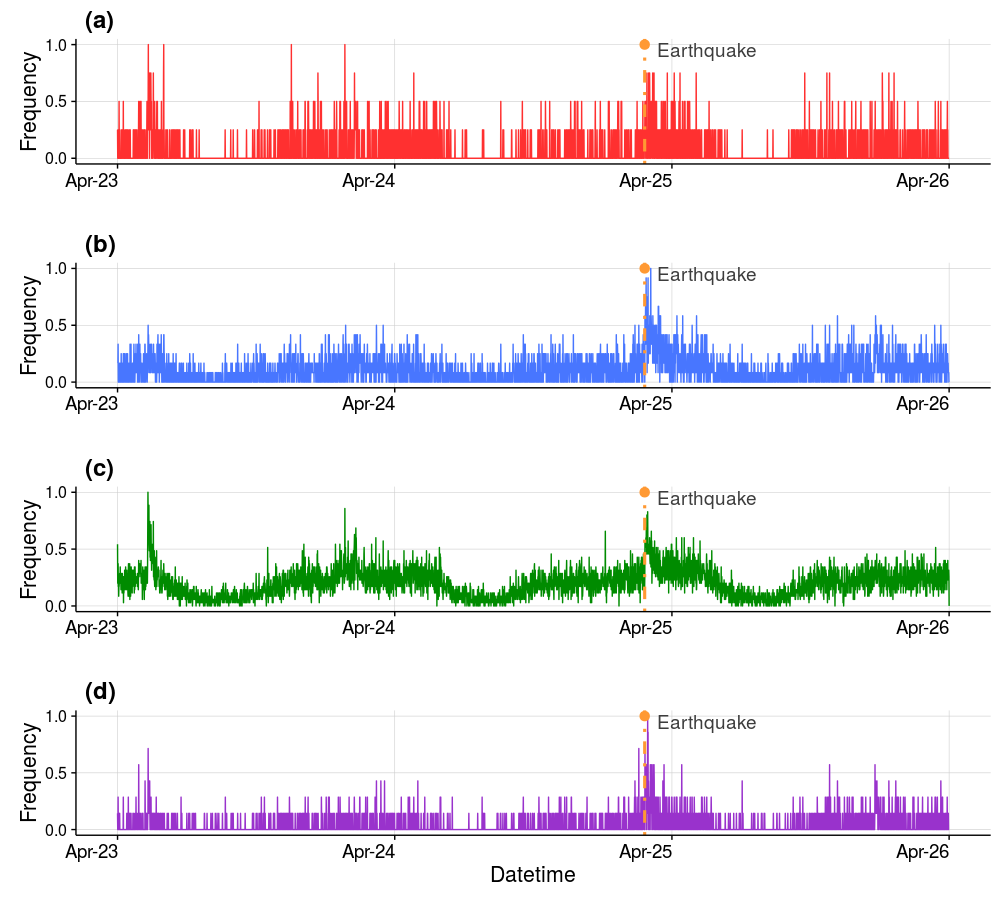
\includegraphics[width=0.5\textwidth]{img/freq_per_minute.png}
	\caption{Normalized Frequency per Minute for Mw 6.9 Chilean Earthquake. (a) \textit{Countrygeo} signal. (b) \textit{Countrytxt} signal.(c) \textit{Countryusr} signal. (d) \textit{Countrytxt-usr} signal.}
\end{figure}


\section{Results and Discussion}

We compare signals when the earthquake occurs. In all cases, signals detect a new emergency situation except the \textit{countrygeo} signal having lower frequency, but represent the exact place where from the message was sent. This result is due to small portion of users using GPS coordinates when sharing a message (about to three per cent or less). The other signals correctly detect  a new emergency situation because its maximum values coincide with an earthquake's datetime, which can be explained by an unusual high-impact event that affect in country-level.

However, the signals that represent country-locations in the text message or the location of the user profile, exhibit noise that can generate a burst for other event types. Sometimes these signals have a relative behaviour that depends on the average daily user's activity of country. 

For reducing this noise exhibited by independent features, we combine the \textit{countrytxt} and the \textit{countryusr} signals for generating the \textit{countrytxt-usr} signal. This means that a user with an inferred locality of Chile shares a message that contains an inferred locality of Chile into the text tweet. Moreover, we can consider that a user (probably in Chile) shares information of Chile in his message, thus, the user cares about things that happen in Chile.

\subsection{Characterization of the Signals}

We characterize an emergency situation by using \textit{inter-arrival times} between consecutive social media messages within a sub-time series. The inter-arrival time is defined as $d_{i} = t_{i+1} - t_{i}$ where $d_{i}$ denotes the difference between two consecutive social media messages $i$ and $i+1$ that arrived in moments $t_{i}$ and $t_{i+1}$, respectively.

Using the \textit{countrytxt-usr} signal, which detect a new emergency situation and has less noise than other signals, we characterize and compare two different sub-time series within of the event. For these tasks, we extract messages one hour before earthquake and messages 10 minutes after earthquakes (Figure \ref{interarrival}). 
\begin{figure}[h]
	\centering
	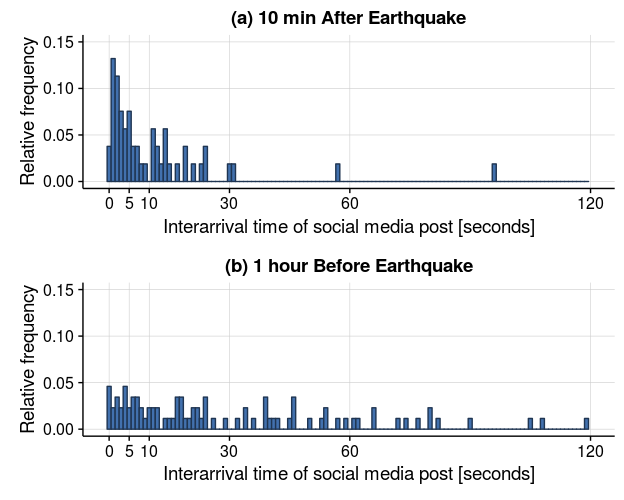
\includegraphics[width=\columnwidth]{img/interarrival.png}
	\caption{Inter-arrival Time Before and During Mw 6.9 Chilean Earthquake}
	\label{interarrival}
\end{figure}

On the one hand, when an unpredicted emergency situation occurs, the urgency of messages can be represented on the first bins, where at least $60$ per cent of the messages have an inter-arrival time $d_{i} < 10$ seconds (Figure \ref{interarrival}.a). Therefore, we learn that when people share messages about a situation on a country, their location usually corresponds with said country.
\\
On the other hand, considering a sub-time series before an earthquake, bins are spread and $28$ per cent of the messages have an inter-arrival time $d_{i} < 10$ seconds (Figure \ref{interarrival}.b). Thus, users in the same country are not simultaneously affected by the same spatio-temporal event and do not share their current location in the message.

\section{Conclusions}
Detecting an emergency situation without using a specific-domain of keywords is important because training data is hard work for researchers. We presented a proposal for detecting this event type using only locations associated with the country. These locations, unlike keywords, do not change over time and do not emerge spontaneously as new terms during an emergency situation.

In the future, we will to include a fine-grained hierarchy for each location which contains country-state-city level with the aim of examining local impact in the first phase after an event. Also, we will compare our approach with keyword-based methods for detecting emergency situation, for example, \cite{kumar2011tweettracker} and \cite{cameron2012emergency}. For this task, we will use public datasets that are generated by \cite{imranaidr2014} or TREC 2011 microblog track. Furthermore, we will inspect the most frequent key phrases and hashtags in the tweets in the burst identified by our method.

\section{Acknowledgments}

I would like to thank my supervisors, Barbara Poblete and Jaime Campos for their supports. We thank ACM SIGIR for the awarded scholarship for participating in ESSIR 2017 and the FDIA Symposium.

\begin{thebibliography}{9}

%\bibliographystyle{chicago}
%\bibliography{bio}

\bibitem[\protect\citeauthoryear{Ashktorab, Brown, Nandi, and
	Culotta}{Ashktorab et~al.}{2014}]{ashktorab2014tweedr}
Ashktorab, Z., C.~Brown, M.~Nandi, and A.~Culotta (2014).
\newblock Tweedr: Mining twitter to inform disaster response.
\newblock {\em Proc. of ISCRAM\/}.

\bibitem[\protect\citeauthoryear{Cameron, Power, Robinson, and Yin}{Cameron
	et~al.}{2012}]{cameron2012emergency}
Cameron, M.~A., R.~Power, B.~Robinson, and J.~Yin (2012).
\newblock Emergency situation awareness from twitter for crisis management.
\newblock In {\em Proceedings of the 21st International Conference on World
	Wide Web}, pp.\  695--698. ACM.

\bibitem[\protect\citeauthoryear{Imran, Castillo, Lucas, Meier, and
	Vieweg}{Imran et~al.}{2014}]{imranaidr2014}
Imran, M., C.~Castillo, J.~Lucas, P.~Meier, and S.~Vieweg (2014).
\newblock Aidr: Artificial intelligence for disaster response.
\newblock In {\em Proceedings of the companion publication of the 23rd
	international conference on World wide web companion}, pp.\  159--162.
International World Wide Web Conferences Steering Committee.

\bibitem[\protect\citeauthoryear{Kumar, Barbier, Abbasi, and Liu}{Kumar
	et~al.}{2011}]{kumar2011tweettracker}
Kumar, S., G.~Barbier, M.~A. Abbasi, and H.~Liu (2011).
\newblock Tweettracker: An analysis tool for humanitarian and disaster relief.
\newblock In {\em ICWSM}.

\bibitem[\protect\citeauthoryear{Olteanu, Castillo, Diaz, and Vieweg}{Olteanu
	et~al.}{2014}]{olteanu2014}
Olteanu, A., C.~Castillo, F.~Diaz, and S.~Vieweg (2014).
\newblock Crisislex: A lexicon for collecting and filtering microblogged
communications in crises.
\newblock In {\em ICWSM}.

\end{thebibliography}

\end{document}
